\chapter{Metodologia}
\label{chap:metodologia}

\section{Princípios da Metodologia}
\label{sec:principios}

Esse presente trabalho em essência é de cunho criativo. Criativo no que diz respeito a procura de uma solução para um problema que tange vários domínios de conhecimentos e, como também, a solução deverá ser de caráter inovador no sentido de haver poucos trabalhos encontrados correlacionados a esse mesmo. A solução, para atingir os objetivos desse trabalho, deverá ser única.

Diante da grande dificuldade em propor algo inovador diante de muitos avanços técnico-científicos e a insegurança de não poder resolver efetivamente o problema, o pensamento filosófico por trás da metodologia considerará uma abordagem não-linear e complexa.

A não-linearidade e a complexidade são atributos chaves para a criatividade. A não-linearidade ocorre inequivocadamente ao longo de toda a construção da solução. Portanto no início do trabalho não houve nenhuma segurança de que a solução seria concretizada ocasionando numa inviabilidade na definição de cronograma. Dado essas condições a taxa de produção intelectual variou muito ocorrendo dias de improdutividade e desesperanças a dias de pura criativiade e confiança.

O processo criativo em essência é complexo \cite{criatividade}. Ele converge diretamente com a teoria da complexidade de Edgar Morin \cite{morin}. Assim como conjecturado pelas pesquisadoras Olzeni Ribeiro e Maria Moraes \cite{criatividade}: a criatividade é complexa e transdisciplinar pois ``entendendemos que a criatividade também é fruto de uma tessitura comum que não separa sujeito, objeto e processo; que não separa sujeito, campo e domínio, como proposto por Mihaly Csiskzentmihalyi; que pode ser compreendida como uma emergência, fruto de um processo interno ao sujeito e que se revela a partir de uma trama energética, informacional ou material que integra fenômenos de natureza biológica, psicológica, social, cultural e espiritural, produto de interações organizacionais complexas constitutivas das várias tramas da vida. A criatividade é fruto de um sentir, pensar e agir em movimento fluente, a partir da atuação do sujeito sobre um objeto ou produto criativo.''

Um exemplo prático de elementos pertencentes a subjetividade do autor na solução é o conhecimento musical transferido para as redes neurais. Tais conhecimentos foram adquiridos por experiências empíricas do autor no domínio da música e de sua visão sobre a mesma.

A criatividade também possui em sua composição a transdisciplinaridade. Esse termo é empregado para o último patamar que conhecemos hoje sobre as relações entre disciplinas e domínios de conhecimento. Conceitua-se como tal um processo que transcende as disciplinas, que está entre, além e através das disciplinas. Nesse trabalho foram investigados vários domínios de conhecimento como a engenharia, matemática, neurociências, psicologia, música e computação. Para ilustrar melhor a dinâmica da transdisciplinaridade segue uma figura ilustrativa do modelo de Jantsch \cite{jantsh}:

\begin{figure}[h]
	\centering
		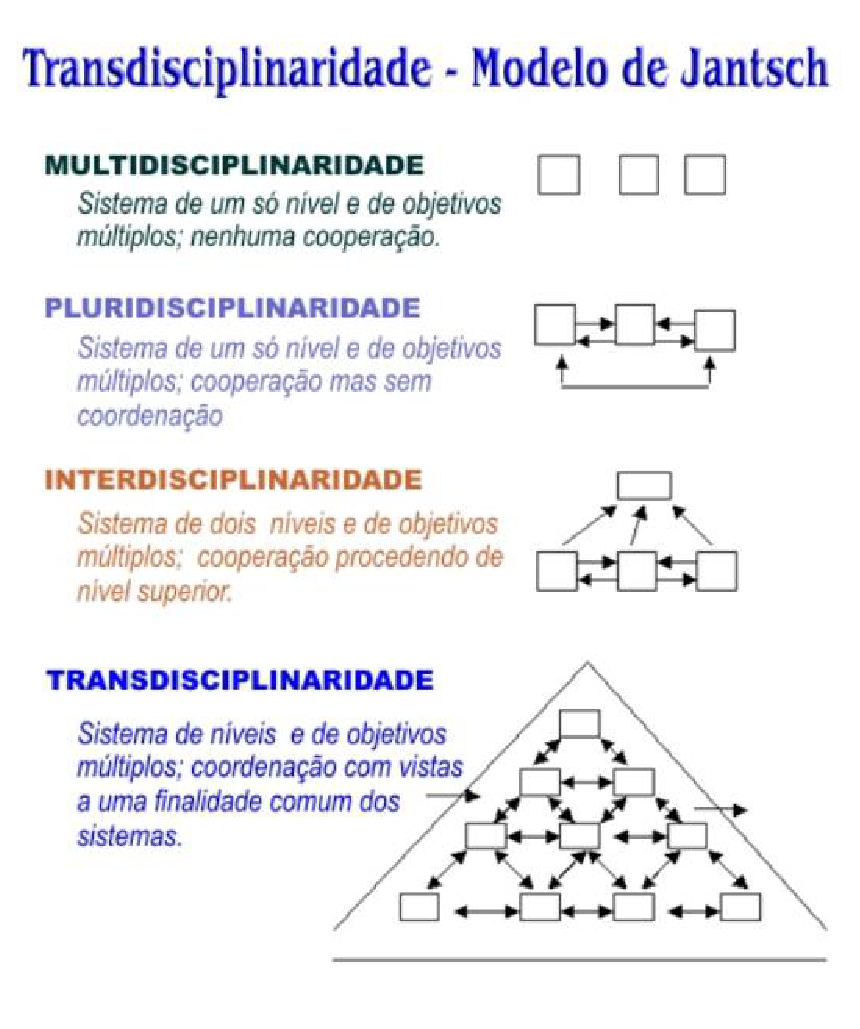
\includegraphics[keepaspectratio=true,scale=0.7]{figuras/trans.eps}
	\caption{Modelo de Jantsch}
\end{figure}

Um outro elemento fundamental para o processo criativo, efetivado empiricamente nesse trabalho, é a presença de uma pessoa confindente, crítica e facilitadora das ideias do autor. Nesse caso essa pessoa foi o professor Dr. Henrique Moura. Esse aspecto é considerado importante pois é apontado também em outras obras como o Mentes Criativas (autor Ph.D. Howard Gardner, criador da teoria das múltiplas inteligências) \cite{gardner}. Essa obra destaca esse padrão nos trabalhos de Freud, Einstein, Picasso, Stravinsky, Eliot, Graham e Gandhi. Esse aspecto se correlaciona muito bem com o papel de um Product Owner na abordagem do Srum que possui uma posição de redirecionar o desenvolvimento de tal forma que possa agregar valor ao produto final \cite{PO}.

Tais conceitos estão presentes no cerne das metodologias ágeis de desenvolvimento de software. Esse fato é devido pois nas mesmas há o uso de práticas com o foco no ser humano para produzir um software único \cite{agile}.

\section{Referencial da Metodologia Científica}
\label{sec:referencialmetodocientifico}

Para a construção da prova conceitual e prática da solução foi adotado como base também o método científico. Segue um fluxo de atividades que foram praticadas \cite{metodo}:

\begin{figure}[h]
	\centering
		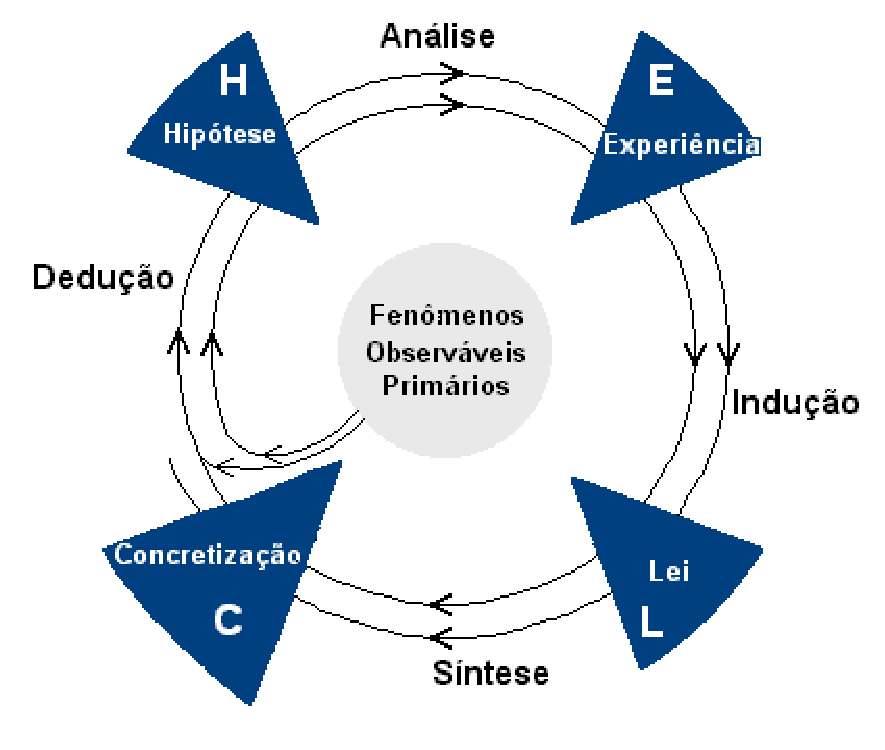
\includegraphics[keepaspectratio=true,scale=0.7]{figuras/metodologia.eps}
	\caption{A praxis científica}
\end{figure}

Através de alguns fenômenos observados, dedutivamente foram levantadas hipóteses como por exemplo: se olhando um espectro de frequências eu consigo dizer qual acorde que é, logo, o computador poderá fazer isso. Levantada essa hipótese, várias experiências foram analisadas como por exemplo o uso de derivadas para a dectecção de picos no espectro de frequências. Através de várias experiências foram feitas induções consolidando um algorítmo de deteccção de picos formando, assim, uma lei procedural para o computador executar. Após foi implementado essa solução numa linguagem de programação para a concretização funcional.

\section{Linguagem de Programação}
\label{sec:linguagemprogramacao}

Existem algumas ferramentas para muitas linguagens de programação que focam processamento de sinais. Uma delas é uma biblioteca em C++ desenvolvida por David Weenink chamada Mel Frequency Cepstral Coefficients (MFCC) \footnote{http://kaldi.sourceforge.net/feat.html\#feat\_mfcc}. Ela dá suporte a extração de dados de arquivos, cálculo da transformada de fourier (FFT) e seu respectivo espectro de energia e cálculo da transformada de cosseno. Uma outra vantagem do uso dela é a linguagem de programação C++ que é bastante rápida em relação ao Java, Ruby e Python. Porém ela não dá suporte a estruturas de álgebra linear e cálculos estatísticos como operação de correlação.

Em vista das necessidades expostas, a linguagem de programação/ferramental escolhida para o trabalho é o Scilab \footnote{http://www.scilab.org/scilab/about}. Scilab é um software científico para computação numérica com sintaxe idêntica ao do Matlab. Essa escolha foi feita primeiramente por tratar de ser um software voltado para aplicações científicas e numéricas, que possuem um viés voltado para os axiomas da álgebra linear. Além disso, essa plataforma possui um conjunto de ferramentas para visualização de gráficos, pacotes de fórmulas matemáticas pré-programadas e estruturas de dados voltadas para a análise numérica. Ela possui uma característica de ser interpretada e dinamicamente tipada.

Além de ter todas as vantagens já citadas, ela é livre com licensa CeCILL (parcialmente permissiva aderente com os tipos GPL). Possui uma comunidade de desenvolvimento ativa com boas práticas de qualidade interna de software como controle de versão GIT, presença de testes unitários e integração contínua com o via software Jenkins \footnote{http://www.scilab.org/development/quality{\_}assurance}.
